GitHub offers a bunch of browser-based tools supporting code review and comments.
Jonathan now prefers this method of providing feedback rather than writing comments in files.
One merit is that the history of feedback persists without cluttering up active code.
Another is that threaded conversations are much cleaner than writing back-and-forth within code.

\subsection{Code review process}\label{code_review_process}
Given a task, the default process for writing code and submitting it for review is the following:
\begin{enumerate}
\item Create a new branch when you create a new task (\href{https://github.com/gslab-econ/ra-manual/wiki/Tasks}{G\&S}: ``The assignee should create a separate git branch for each task that involves code or output stored in the repository.'')
\item Commit your work on this new branch. A complete task includes a \texttt{Makefile}.
\item In addition to creating a \texttt{code} folder, write a \texttt{readme.md} in the task folder that explains what it does.
\item Submit a pull request when your code is ready to be reviewed.
\item Team uses the pull request to review code and have a conversation about the task
\item Additional commits are made on the branch in response to discussion and feedback.
\item Finalized task is added to master branch using \href{https://docs.github.com/en/pull-requests/collaborating-with-pull-requests/incorporating-changes-from-a-pull-request/about-pull-request-merges#squash-and-merge-your-commits}{a merge that squashes} the branch's commits.
\end{enumerate}

A reviewer will execute the following steps when reviewing a pull request.

\begin{enumerate}
\item Run \texttt{make} in \texttt{tasks/task\_graph} to create \texttt{task\_flow\_branchdiff.png}
    (Note: in order for the graph to be informative, your branch must be up-to-date with main.)
\item Referencing \texttt{task\_flow\_branchdiff.png},
    delete all input and output folders in the tasks that were created or
    modified on the branch.\footnote{An exception to this rule:
    it would be costly to delete the output folder of \texttt{downloaddata} every time,
    as it bundles all downloads. Instead, only delete the outputs that are relevant to the changes
    on the branch.}
\item Run \texttt{make} in the tasks that were created or modified on the branch.
\item Run \texttt{make} in the logbook folder if an entry was created or its inputs were modified.
\item Run \texttt{make} in the paper or slides folders if they or their inputs were modified.
\item Repeat (2)-(5) until there are no errors.
\end{enumerate}

The person submitting the request---who
will select themselves as the ``assignee'' on GitHub---should
also go through these steps before submitting a pull request
to catch common bugs in advance.
It is ideal if the reviewer can immediately focus on the substance of the code
and not have to spend time notifying the assignee about errors in scripts or \texttt{Makefile}s.

We use GitHub actions to automatically check
that Makefiles are valid when a pull request is submitted.
You can see the status of these checks on the GitHub pull request page.
If any fail,
fix the mistakes and then re-request review to run the checks again.
Note that you can also run the checks manually by executing the shell
scripts in \texttt{tasks/check\_makefiles}.
Similarly, running \texttt{make} in \texttt{tasks/maintenance} flags scripts and \texttt{Makefile}s that
violate best practices or our style preferences.

When reviewing a pull request,
you should check the code for correctness and efficiency.
Consult the logbook entry on writing code (\ref{sec:writing-code}) for our style preferences.

\subsection{Notes on the process}
These notes are for the assignee,
but the reviewer should also be checking for compliance with these guidelines.

\subsubsection{Commit data reports}
We have tools in place to generate reports that summarize the characteristics of datasets.
In Stata, datasets should be saved using the \texttt{save\_data} command,
as it automatically generates these reports.
The command has the additional benefit of enforcing that datasets have unique,
non-missing keys which are specified with the \texttt{key()} option
 (see the section dedicated to keys in \href{https://web.stanford.edu/~gentzkow/research/CodeAndData.pdf}{Gentzkow and Shapiro's Code and Data} for why this is a sensible requirement for your datasets).
We wrote an \texttt{awk} script that generates similar reports for CSV files.
To use it, run \texttt{make ../report/[file].csv.log}
in the code folder of the task that creates the CSV file.
You should specify the paths for all the reports that will be created by awk
in a \texttt{reports} recipe in the \texttt{Makefile}.
We hope to have tools similar to \texttt{save\_data} and the \texttt{awk} script
for \texttt{R} and \texttt{Python} in the future. % TODO: Describe how to use these tools once we have them.

By committing the reports to GitHub, we can track changes to datasets.
This practice allows us to quickly identify the reason for a change in results,
either when run by our collaborators on a different machine or by someone
who is replicating our work.
Ensure that you have committed the reports for all datasets
that you have created or modified before submitting a pull request.

\subsubsection{Avoid large pull requests if possible}
Similar to the rule that more commits are better than fewer commits,
it is better to have modest-sized pull requests at higher frequency
than gargantuan pull requests at lower frequency.
Smaller pull requests are not only more convenient for the reviewer;
they also reduce merge conflicts
and make it easier to track down bugs later.
Both commits and pull requests require brief messages or titles,
which capture the changes that occurred.
The brevity of the messages hints that commits and pull requests are designed
to make a single change and to process the set of changes related to a single task, respectively.

\subsubsection{Wait for approval before merging into main}
Sometimes it makes sense to have multiple reviewers for a pull request.
For example, in a pull request that adjusts content within the paper,
the authors will likely all want to sign off on the changes.
You should wait for the reviewers' consensus approval before merging into main.

\subsubsection{Resolve merge conflicts}
During this process, you may be told that there are merge conflicts between
your branch and main that must be addressed before the pull request can be completed.
This message indicates that your branch and main have made changes to the same files.
You can easily resolve these conflicts from the terminal.
First, run \texttt{git pull} on the main branch to get the latest changes.
Then, switch to your branch and run \texttt{git merge main}.
Git lists the files that contain these conflicts
(see progress with \texttt{git status}), marks the problematic lines within the files,
and will not complete the merge until you manually
select the changes that you want to keep.
See this guide from GitHub for
\href{https://help.github.com/articles/resolving-a-merge-conflict-using-the-command-line/}{resolving merge conflicts using the command line}.
Text editors often have tools to assist in resolving merge conflicts.
See here for VS Code's \href{https://code.visualstudio.com/docs/editor/versioncontrol#_merge-conflicts}{merge conflict resolution interface}.

\subsubsection{Handle untracked files}
\texttt{git status} informs you of any untracked files sitting on your branch.
Untracked files should be committed if you want to include them in the pull request.
Sometimes these files can prevent you from executing a merge
(e.g., the files are artifacts from your work on another branch, and
the merge would overwrite your local copies).
If a file has relevant changes, you should commit it before completing the merge.
If you simply want to take the copy of the file from the branch that you are merging
in---since you did not edit it on your branch, or it is no longer relevant---you
can safely delete it.
You can easily delete untracked files with \texttt{git clean}.
Run \texttt{git clean -n} to see what files will be deleted,
and then run \texttt{git clean -f} to delete them.

\subsubsection{Add packages to setup\_environment}
If you use a package in Stata, R, Python, or Julia,
you should add it to the appropriate \texttt{setup\_environment} file before
submitting a pull request.
This ensures that the code will run on other machines when proper setup
instructions are followed.

\subsection{Commenting on commits}

\subsubsection{Comment on a file}
Jonathan wrote two comments about data visualization on commit \texttt{abf9191}.
Scrolling through the commit webpage, Jonathan clicks on ``comment'' for \texttt{output/figures/summarystats/device\_byzip.eps} and says the following:
\begin{center}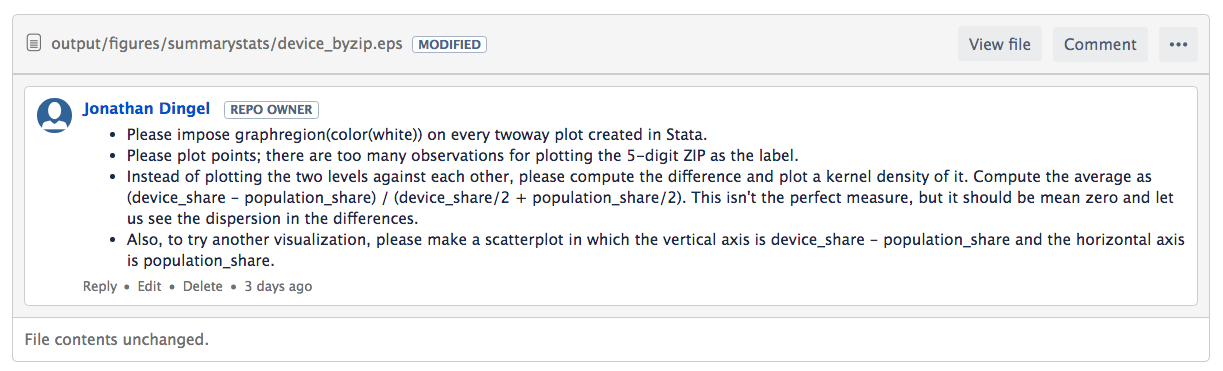
\includegraphics[width=.8\textwidth]{./figures/workflow/BitBucket_screenshot_commenting1.png}\end{center}
Ningyin can reply to the comment to ask for clarification, and Jonathan can link to this commit comment when assigning tasks.

\subsubsection{Comment on a line}
You can also write comments on individual lines of a file.
Jonathan spotted a ``force'' option on line 99 of \texttt{code/gen\_census\_data.do} and wrote a comment seeking clarification.
He embeds his code suggestion as part of the comment, complete with GitHub's language-specific syntax highlighting.
\begin{center}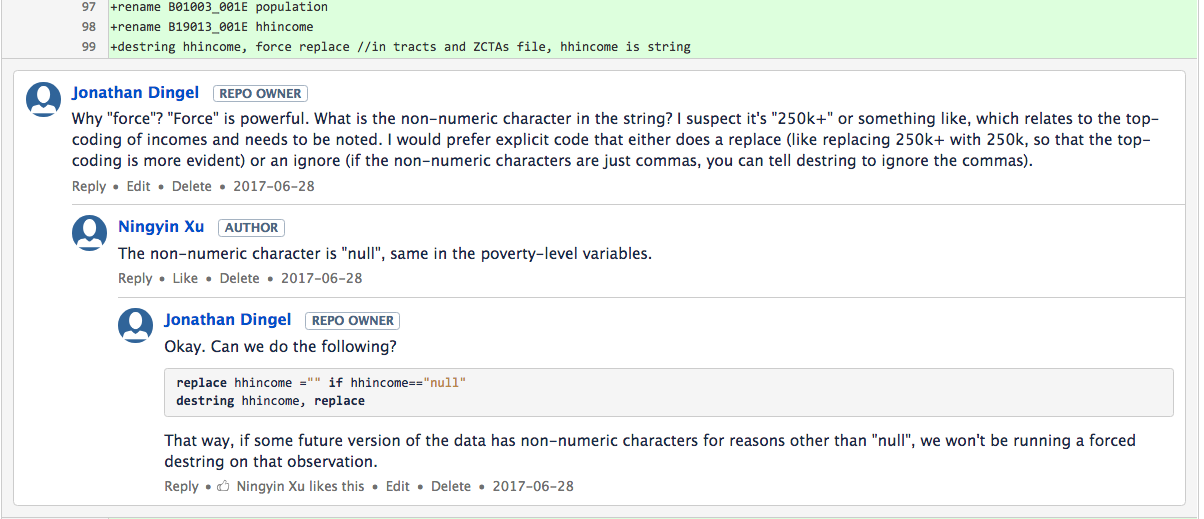
\includegraphics[width=\textwidth]{./figures/workflow/BitBucket_screenshot_commenting2.png}\end{center}

\subsection{Submit a GitHub pull request review}
When making your first comment, select the ``Start a review'' option to initiate a review.
You can track the files that you have reviewed by clicking on the ``Viewed'' button
in the top right corner of the file in the ``Files changed'' tab.
After you have reviewed all files,
click the ``Review changes'' button in the top right corner of the page,
write any summary comments, and select ``Approve'' or ``Request changes''.
All the comments that you made will then be submitted, and the assignee will be notified.
If you are interested in reviewing pull requests outside a browser,
\href{https://cli.github.com/}{GitHub command line} has commands for
reviewing pull requests from the terminal
(and other GitHub operations that are usually done from the browser).
There are also text-editor plugins that allow you to review pull requests,
such as \href{https://marketplace.visualstudio.com/items?itemName=GitHub.vscode-pull-request-github}{GitHub Pull Requests and Issues} for VS Code.
